\documentclass[11pt]{article}



\def\changemargin#1#2{\list{}{\rightmargin#2\leftmargin#1}\item[]}
\let\endchangemargin=\endlist 

%------------------------------------------------------------------
% PROBLEM, PART, AND POINT COUNTING...

% Create the problem number counter.  Initialize to zero.
\newcounter{problemnum}

% Specify that problems should be labeled with arabic numerals.
\renewcommand{\theproblemnum}{\arabic{problemnum}}


% Create the part-within-a-problem counter, "within" the problem counter.
% This counter resets to zero automatically every time the PROBLEMNUM counter
% is incremented.
\newcounter{partnum}[problemnum]

% Specify that parts should be labeled with lowercase letters.
\renewcommand{\thepartnum}{\arabic{partnum}}

% Make a counter to keep track of total points assigned to problems...
\newcounter{totalpoints}

% Make counters to keep track of points for parts...
\newcounter{curprobpts}		% Points assigned for the problem as a whole.
\newcounter{totalparts}		% Total points assigned to the various parts.

% Make a counter to keep track of the number of points on each page...
\newcounter{pagepoints}
% This counter is reset each time a page is printed.

% This "program" keeps track of how many points appear on each page, so that
% the total can be printed on the page itself.  Points are added to the total
% for a page when the PART (not the problem) they are assigned to is specified.
% When a problem without parts appears, the PAGEPOINTS are incremented directly
% from the problem as a whole (CURPROBPTS).


%---------------------------------------------------------------------------


% The \problem environment first checks the information about the previous
% problem.  If no parts appeared (or if they were all assigned zero points,
% then it increments TOTALPOINTS directly from CURPROBPTS, the points assigned
% to the last problem as a whole.  If the last problem did contain parts, it
% checks to make sure that their point values total up to the correct sum.
% It then puts the problem number on the page, along with the points assigned
% to it.

\newenvironment{problem}[1]{
% STATEMENTS TO BE EXECUTED WHEN A NEW PROBLEM IS BEGUN:
%
% Increment the problem number counter, and set the current \ref value to that
% number.
\refstepcounter{problemnum}
%
% Add some vspace to separate from the last problem.
\vspace{0.15in} \par
%
\setcounter{curprobpts}{#1} \setcounter{totalparts}{0}	% Reset counters.
%
% Now put in the "announcement" on the page.
\noindent{\Large \bf Question \theproblemnum. \normalsize ({\it \arabic{curprobpts} point\null\ifnum \value{curprobpts} = 1\else s\fi}\/)}
}{
% STATEMENTS TO BE EXECUTED WHEN AN OLD PROBLEM IS ENDED:
%
% If no parts to problem, then increment TOTALPOINTS and PAGEPOINTS for the
% entire problem at once.
\ifnum \value{totalparts} = 0
	\addtocounter{totalpoints}{\value{curprobpts}}	% Add pts to total.
	\addtocounter{pagepoints}{\value{curprobpts}}	% Add pts to page total.
%
% If there were parts for the problem, then check to make sure they total up
% to the same number of points that the problem is worth. Issue a warning
% if not.
\else \ifnum \value{totalparts} = \value{curprobpts}
	\else \typeout{}
	\typeout{!!!!!!!   POINT ACCOUNTING ERROR   !!!!!!!!}
	\typeout{PROBLEM [\theproblemnum] WAS ALLOCATED \arabic{curprobpts} POINTS,}
	\typeout{BUT CONTAINS PARTS TOTALLING \arabic{totalparts} POINTS!}
	\typeout{}
	\fi
\fi
}


%---------------------------------------------------------------------------


% The \newpart command increments the part counter and displays an appropriate
% lowercase letter to mark the part.  It adds points to the point counter
% immediately.  If 0 points are specified, no point announcement is made.
% Otherwise, the announcement is in scriptsize italics.

\newcommand{\newpart}[2]{
\refstepcounter{partnum}	% Set the current \ref value to the part number.
\begin{changemargin}{0in}{0in}
  \noindent\textbf{\theproblemnum.\thepartnum}~(\textit{#1 points}): 
  \textit{ #2}
\end{changemargin}
\addtocounter{totalparts}{#1}	% Add points to totalparts for this problem.
\addtocounter{pagepoints}{#1}	% Add points to total for this page.
\addtocounter{totalpoints}{#1}	% Add points to total for entire test.
}

\newcommand{\answerpart}[1]{
\begin{changemargin}{0.25in}{0in}
\noindent \textbf{Answer:} {#1}
\end{changemargin}	
}

\newcommand{\answer}[1]{
\textbf{Answer:} {#1}
}



%---------------------------------------------------------------------------



% Just in case you want to skip some numbers in your test...

\newcommand{\skipproblem}[1]{\addtocounter{problemnum}{#1}}



%---------------------------------------------------------------------------


% The \showpoints command simply gives a count of the total points read in up to
% the location at which the command is placed.  Typically, one places one
% \showpoints command at the end of the latex file, just prior to the
% \end{document} command.  It can appear elsewhere, however.

\newcommand{\showpoints}
{
\typeout{}
\typeout{====> A TOTAL OF \arabic{totalpoints} POINTS WERE READ.}
\typeout{}
}


%---------------------------------------------------------------------------



\usepackage{fullpage} \usepackage{graphicx} \usepackage[english]{babel}
\usepackage[latin1]{inputenc} \usepackage{times} \usepackage[T1]{fontenc}
\usepackage{amsmath} \usepackage{amssymb} \usepackage{color}
\usepackage{hyperref}

\newcommand{\argmax}{\mathop{\arg\max}}
\newcommand{\deriv}[1]{\frac{\partial}{\partial {#1}} }
\newcommand{\dsep}{\mbox{dsep}} \newcommand{\Pa}{\mathop{Pa}}
\newcommand{\ND}{\mbox{ND}} \newcommand{\De}{\mbox{De}}
\newcommand{\Ch}{\mbox{Ch}} \newcommand{\graphG}{{\mathcal{G}}}
\newcommand{\graphH}{{\mathcal{H}}} \newcommand{\setA}{\mathcal{A}}
\newcommand{\setB}{\mathcal{B}} \newcommand{\setS}{\mathcal{S}}
\newcommand{\setV}{\mathcal{V}} \DeclareMathOperator*{\union}{\bigcup}
\DeclareMathOperator*{\intersection}{\bigcap} \DeclareMathOperator*{\Val}{Val}
\newcommand{\mbf}[1]{{\mathbf{#1}}} \newcommand{\eq}{\!=\!}
\newcommand{\cut}[1]{}
\newcommand{\update}[1]{\textcolor{blue}{[#1]}}

\begin{document}

{\centering \rule{6.3in}{2pt} \vspace{1em} {\Large CS688: Graphical Models -
Spring 2020\\ Assignment 2\\ } \vspace{1em}
Assigned: Thursday, Feb 27th. Due: Friday, Mar 13rd, 5:00pm\\ \vspace{0.1em} \rule{6.3in}{1.5pt}
}\vspace{1em}


\textbf{General Instructions:} 
Please upload {\em\bf two items} to \textit{Gradescope} (\url{https://www.gradescope.com/courses/86501}): (1) a report with your answers (\textit{.pdf}), and (2) a zip file with your code (\textit{.zip}).\\
Submit a report with the answers to each question. You are encouraged to typeset your solutions. 
To help you get started, the full \LaTeX source of the assignment is included with the assignment materials. For your assignment to be considered ``on time'', you must upload a zip file containing all of your code to \textit{Gradescope} by the due time.
Make sure the code is sufficiently well documented that it's easy to tell what it's doing. You may use any programming language you like. For this assignment, you may not use
existing code libraries for inference and learning with CRFs or MRFs. If you
think you've found a bug with the data or an error in any of the assignment
materials, please post a question to the discussion forum. Make sure to
list in your report any outside references you consulted (books, articles, web
pages, etc.) and any students you collaborated with.\\ \\
When you submit reports through \textit{Gradescope}, you are supposed to mark what part of the .pdf corresponds to each question. Please note that you will lose credit on this assignment if you fail to do this. \\

\textbf{Academic Honesty Statement:} Copying solutions from external sources
(books, web pages, etc.) or other students is considered cheating. Sharing your
solutions with other students is also considered cheating. Any detected
cheating will result in a grade of 0 on the assignment for all students
involved, and potentially a grade of F in the course. See course policies on the course website.\\

\textbf{Introduction:} In this assignment, you will experiment with different
aspects of modeling, learning, and inference with chain-structured conditional
random fields (CRFs). This assignment focuses on the task of optical character
recognition (OCR). We will explore an approach that bridges computer vision and
natural language processing by jointly modeling the labels of sequences of
noisy character images that form complete words. This is a natural problem for
chain-structured CRFs. The node potentials can capture bottom-up information
about the character represented by each image, while the edge potentials can
capture information about the co-occurrence of characters in adjacent positions
within a word.  \\

\textbf{Code: } You may write code in any language you want, though we suggest a language with convenient numerical libraries such as Python, Matlab, Julia, or R.
We have provided ``suggested pseudocode'' function signatures in \texttt{Latex-Source/functions.txt} as a suggestion for how you could structure your code. \\

\textbf{Data: } The underlying data are a set of $N$ sequences corresponding to
images of the characters in individual words. Each word $i$ consists of $L_i$
positions. For each position $j$ in word $i$, we have a noisy binary image of
the character in the position. In this assignment, we will use the raw
(binary) pixel values of the character images as features in the CRF. The
character images are $20\times 16$ pixels. We convert them into $1\times 320$
vectors. We include a constant bias feature along with the pixels in each
image, giving a final feature vector of length $F=321$. $x^{(i)}_{jf}$ indicates the
value of feature $f$ in position $j$ of word $i$. The provided training and
test files (\texttt{train\_img<i>.txt} and \texttt{test\_img<i>.txt}) list the
character image $\mbf{x}^{(i)}_{j}$ on row $j$ of file $i$ as a $321$-long
space-separated sequence.\footnote{Images are also provided for each training and test word as standard PNG-format files (\texttt{train\_img<i>.png} and
\texttt{test\_img<i>.png}). These are for your reference and not for use in
training or testing algorithms.} The data files are in the column-major format.
Given the sequence of character images

\[ \mbf{x}^{(i)}=[\mbf{x}^{(i)}_{1},...,\mbf{x}^{(i)}_{L_i}]\]
corresponding to test word $i$,
our goal is to infer the corresponding sequence of character labels

\[ \mbf{y}^{(i)}=[y^{(i)}_{1},...,y^{(i)}_{L_i}].\]
To reduce the computational complexity of
exhaustive inference, we will use a limited set of characters corresponding to
the $10$ most frequently used characters in the English language:
\texttt{etainoshrd}. There are thus $C=10$ possible labels for each word position.
The character labels for each training and test word are available in the files
\texttt{train\_words.txt} and \texttt{test\_words.txt}. The figure below shows
several example words along with their images.  

\begin{center}
  \begin{minipage}[t]{1.4in}\centering
    shoot
    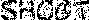
\includegraphics[scale=1]{images/train_img1.png}
  \end{minipage}
  \hspace{1em}
  \begin{minipage}[t]{1.4in}\centering
    indoor
    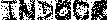
\includegraphics[scale=1]{images/train_img2.png}
  \end{minipage}
  \hspace{1em}
  \begin{minipage}[t]{1.4in}\centering
    three
    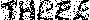
\includegraphics[scale=1]{images/train_img3.png}
  \end{minipage}
  \hspace{1em}
  \begin{minipage}[t]{1.4in}\centering
    trait
    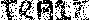
\includegraphics[scale=1]{images/train_img4.png}
  \end{minipage}
\end{center}



\textbf{Model:} The conditional random field model is a conditional model
$P_W(\mbf{y}|\mbf{x})$ of the sequence of class labels $\mbf{y}$ given
the sequence of feature vectors $\mbf{x}$ that depends on a collection of
parameters $W$. The CRF graphical model is shown below for a sequence of length
$4$.\\

\begin{center}
    \centering
    \textbf{Conditional Random Field}\\\vspace{10pt}
    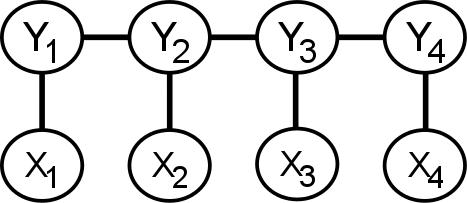
\includegraphics[scale=0.4]{images/crf.png}
\end{center}

The CRF model contains one feature parameter $W^F_{cf}$ for each pair of the $C=10$  character labels and $F=321$ features\footnote{Be careful: The $F$ in $W^F$ is there only to indicate these are "feature parameters". It does not stand for the $F=321$ features. The same is true for the $F$ or $T$ in $W^T$, $\phi^F$ and $\phi^T$ below.}. These parameters thus encode the
"compatibility" between feature values and character labels. The CRF also
contains one transition parameter $W^T_{cc'}$ for each pair of character labels
$c$ and $c'$.  The transition parameters encode the "compatibility" between
adjacent character labels in the word. We parameterize the model in log-space,
so all of the parameters can take arbitrary (positive or negative) real values.
We have one feature potential $\phi^F_j(y_{j},\mbf{x}_{j})$ for each position
$j$ and one transition potential for each pair of adjacent labels
$\phi^T_j(y_{j},y_{j+1})$.
%
\begin{align*}
  \phi^F_j(y_{j},\mbf{x}_{j};W^F) &= \exp \left( \sum_{f=1}^F W^F_{y_{j}f} \, x_{jf}  \right) \\
  \phi^T_{j}(y_{j},y_{j+1};W^T) &= \exp \left(W^T_{y_{j}y_{j+1}} \right)
\end{align*}
%

% For the rest of the assignment, we use $I[\dots]$ as the notation for indicator functions, i.e.\ $I[conditions]$ equals $1$ when $\mathrm{conditions}$ are all met, and $0$ otherwise. For example, $I[y_{j}=c]$ equals $1$ when $y_{j}=c$, and $0$ otherwise. 

Note that these potentials are always positive. Please inspect the data files and
make sure you understand the shapes of each variable and the resulting shapes
of the potentials. As always with undirected model, the joint
distribution must be explicitly normalized, as shown below. In CRF model like this, the normalizing constant depends both on the parameters and the input features. So, for sequences $\mbf{x}$ and $\mbf{y}$ of length $L$,

\begin{align*}
P_{W}(\mbf{y}, \mbf{x})
&=\frac{1}{Z(W)} \prod_{j=1}^{L}\phi^F_j(y_{j},\mbf{x}_{j};W^F) \cdot \prod_{j=1}^{L-1}\phi^T_j(y_{j},y_{j+1};W^T)
       \\
&= \frac{1}{Z(W)}
     \exp\left(\sum_{j=1}^{L_i}\sum_{f=1}^F W^F_{y_j f} \, x_{jf}
     +\sum_{j=1}^{L_i-1}W^T_{y_j y_{j+1}} \right),
\end{align*}\\

\noindent Where $Z(W)$ is the normalizing constant which can be written as

\begin{align*}
Z(W)
&=\displaystyle
         \sum_{\mbf{y}}\sum_{\mbf{x}}\prod_{j=1}^{L}\phi^F_j(y_{j},\mbf{x}_{j};W^F) \cdot \prod_{j=1}^{L-1}\phi^T_j(y_{j},y_{j+1};W^T)\\
&= \displaystyle
     \sum_{\mbf{y}}\sum_{\mbf{x}}\exp\left(\sum_{j=1}^{L}\sum_{f=1}^F
     W^F_{y_{j} f} \, x_{jf}
     +\sum_{j=1}^{L-1} W^T_{y_{j} y_{j+1}}\right).
\end{align*}

\begin{problem}{20} \textbf{Exhaustive Inference:} In this question, you will
  implement simple exhaustive inference for the CRF model. The code packages
  provides a pre-trained model for the OCR task including the feature
  parameters (\texttt{feature-params.txt}) and the label-label transition
  parameters (\texttt{transition-params.txt}). Use these parameters to answer
  the following questions. For grading purposes, make sure to list results
  table rows and/or columns using the character ordering \texttt{etainoshrd}.

\newpart{2} {For the first test word only, compute the node potentials
\[ \phi'(y_{j})=\phi^F_j(y_{j},\mbf{x}_{j};W^F) \]
obtained by conditioning the CRF on the observed image sequence. After conditioning, there is one node potential per position in the test word. Each node potential is a vector with one entry per character label. Report the node potential \textbf{in log space} as a table for each position in the test word.} 

\newpart{2} {Energy is a function which measures the ``goodness'' (or badness) of each possible configuration of the random variables (the lower the engergy, the better the configuration). 
We can define energy as the negative logarithm of (possibly unnormalized) probability. For the first three test words, compute the value of the negative
  energy of the true label sequence after conditioning on the corresponding
  observed image sequence. For sequences $\mbf{x}$ and $\mbf{y}$ of length $L$ this is
  $$-E_W(\mbf{x},\mbf{y})=\sum_{j=1}^{L} \log \phi'(y_{j}) + \sum_{j=1}^{L-1} W^T_{y_{j} y_{j+1}}.$$}

\newpart{6}{For the first three test words, use exhaustive summation over all
possible character label sequences to compute the value of the log partition
function for the CRF model after conditioning on the corresponding observed
image sequence. Report the value you compute.}

\newpart{6}{For the first three test words, compute the most likely joint
labeling (character sequence) word. Report both the labeling and its
probability under the model.}

\newpart{4}{For the first test word only, compute the marginal probability
  distribution over character labels for each position in the word. Report each
  marginal distribution using a table.} 
  
\textbf{Note}: the results may contain very small values, so please report in scientific notation such as \texttt{6.06 e-12} instead of \texttt{0.0}.  If you're having trouble with this,
  try using the ``g'' format code in Python \texttt{str.format} 
  or \texttt{\%g} in \texttt{sprintf}-style formatting (or other methods).
  This may hold for other questions too.

\end{problem}

\begin{problem}{40} \textbf{Sum-Product Message Passing:} In this question, you
  will implement the sum-product inference algorithm for the CRF model. The
  code packages provides a pre-trained model for the OCR task including the
  feature parameters (\texttt{feature-params.txt}) and the label-label
  transition parameters (\texttt{transition-params.txt}). Use these parameters
  to answer the following questions.
 
\newpart{10}{For the first test word only, condition on the observed image
  sequence to obtain a chain-structured Markov network. Compute the \textbf{log-space} messages $m_{1\rightarrow 2}(Y_2)$,
  $m_{2\rightarrow 1}(Y_1)$, $m_{2\rightarrow 3}(Y_3)$,
  $m_{3\rightarrow 2}(Y_2)$. Report the value of each message in a table.}

\newpart{15}{For the first test word only, use the computed messages to
  compute marginal probability distributions. 
  Report single variable marginals over each position in the word as a table. 
  Represent pairwise marginals over each adjacent node pairs as three tables, 
  and report only the $3\times 3$ block of entries between the labels ``t,a,h'' in each table.}

\newpart{15}{Generalize the steps given above to compute the single variable
  and pairwise marginal probabilities for any sequence of input images. Apply
  your completed algorithm to compute the marginal probability distribution
  over the character labels given the image sequences for each word in the test
  set. For each position in each test word, predict the character with maximum
  probability. List your predictions for the first five test sequences.  In
  addition, use the true character labels in \textit{test\_words.txt} to
  compute the average character-level accuracy over the complete test set. Report
  the accuracy that you find to three decimal places.}

\end{problem}

\begin{problem}{34} \textbf{Maximum Likelihood Learning Derivation:} In this
  problem, you will derive the maximum likelihood learning algorithm for
  conditional random field models.

\newpart{8}{Write down the average log likelihood function for the CRF given a
  data set consisting of $N$ image sequences $\mbf{x}^{(i)}$ and label sequences
  $\mbf{y}^{(i)}$.} 

\newpart{8}{Derive the derivative of the average log likelihood function with
  respect to the feature parameter $W^F_{cf}$. Show your work.} 

\newpart{8}{Derive the derivative of the average log likelihood function with
  respect to the transition parameter $W^T_{cc'}$. Show your work.} 

\newpart{8}{ Explain how, as a byproduct of the sum-product algorithm's
computation of the single-variable and pairwise marginal probabilities, you can
efficiently compute both the value of the log-likelihood function and the
values of the above derivatives.}

\newpart{2}{Using a data set consisting of the first 50 training data cases only, compute the average log likelihood of the true label sequences given the image sequences using the supplied model parameters.}

\newpart{0}{Using a data set consisting of the first 50 training data cases
only, compute the derivative with respect to each model parameter of the
average log likelihood of the true label sequences given the image sequences
using the supplied model parameters. There is nothing to hand in for this
question, but we will provide the solution to help you debug your code. These
files are in the model folder and called feature-gradient.txt and
transition-gradient.txt.}
\end{problem}


\begin{problem}{6} \textbf{Numerical Optimization Warm-Up:} In the next
  assignment, you will implement the above learning algorithm using a numerical
  optimizer to maximize the log likelihood. In this question, you will
  experiment with optimizing a basic function.

\newpart{3}{Consider the objective function $f_w(x,y) = -(1-x)^2 -
100(y-x^2)^2$. Derive the derivatives of $f(x,y)$ with respect to $x$ and $y$
(the gradient function). Show your work.  } 

\newpart{3}{Select a numerical optimizer for the programming language you are
  using. If you haven't used it previously, study its documentation carefully.
  Implement the objective function and the gradient function in the form
  required by your numerical optimizer. Write code to use the optimizer to
  \textbf{maximize} $f(x,y)$. Report both the location of the maximum and the
  value of the objective function at the maximum. 
} 

Note that most optimization functions minimize by default (e.g. functions in the \texttt{scipy.optimize module}).
Getting this wrong is a very common bug.

\end{problem}


\showpoints
\end{document} 
